% Great animation about protons going through the CERN accelerator complex.
% https://www.youtube.com/watch?v=FLrEghnKncA
\chapter{THE LARGE HADRON COLLIDER}
\label{ch:lhc}

% OUTLINE
\section{Motivation}
Although the SM (Chapter~\ref{ch:theory}) has shown to be an astoundingly accurate framework so far, it must continue to be scrutinized by the barrage of measurements that either confirm or contradict its predictions.
% cross-examined
Interestingly, a recent measurement of the mass of the \PW boson has shown significant deviation from SM predictions, with a sensitivity of 7$\sigma$ TODO:ref.
After all, undeniable fact comes from the reproducible results obtained from \emph{measurement}---not from some theoretical model which \emph{may} or \emph{may not} describe reality.
Whenever the predictions of a model directly contradict the results from measurement, the model must necessarily be cast aside and replaced by one whose predictions concur with the results of measurement.
% the truth of Nature

So how \emph{are} measurements obtained in the realm of particle physics?
% be continuously tested for its accuracy.
% Must be shaken by the results of experiment to see if its foundation is stable.
% So far, it has upheld against the onslaught of measurements but must be continuously tested for accuracy.
% , it does not explain many phenomena observed in the universe, as discussed in ().
% Although the SM (Chapter~\ref{ch:theory}) is an astoundingly accurate framework, it does not explain many phenomena observed in the universe, as discussed in ().
% As discussed in TODO:PROBLEMS WITH SM, there is observed physics that has not yet been explained in a coherent theoretical and mathematical framework.
% There are currently many searches for physics \emph{beyond the standard model} (BSM) which may explain certain observed physical phenomena that .
% robust, elegant, and accurate (so far), 
% perhaps there is physics beyond the SM (BSM).
% After all, the truth of Nature comes from the results of measurements---not from mathematical and theoretical models.
% Although the standard model (SM) of particle physics  is rather elegant
% and  for the physical phenomena that it does explain.
Modern day physicists study the fundamental constituents of matter and their interactions by using state-of-the-art technologies combined with time-tested methodologies:
%  is to do it the same way humans have been doing it for centuries:
by smashing tiny bits of matter together to turn them into even \emph{tinier} bits.
Such is the purpose of the world's largest and most powerful particle accelerator---the Large Hadron Collider (LHC).

\section{The LHC at CERN}
% The circular LHC ring straddles the Franco-Swiss border, approximately 100\meter below the surface of the earth
% (Fig.~\ref{fig:lhc_and_boosters}, Left).
% The ring itself has a circumference of 26.7\Km, making its inscribed area (56.7$\Km^{2}$) almost four times greater than the area of the neighboring city of Geneva (15.9$\Km^{2}$).
% This machine is not only a particle accelerator but also a proton-proton (\pp) collider, sending one beam of protons travelling clockwise and the other beam counterclockwise around the ring. 
TODO:cleanup.
Deep beneath the surface of the earth (50--175\meter), the LHC straddles the border shared by France and Switzerland.
Sandwiched between the scenic Jura mountains to the northwest and the sprawling city of Geneva (French: Genève) to the southeast (Fig.~\ref{fig:lhc_on_map_and_complex}, Left), .
To illustrate the enormous circumference (26.659\Km) the sheer size of this circular accelerator, Fig.~\ref{fig:lhc_on_map_and_complex} (Left) shows the LHC drawn on a map to .
% Map and CERN complex.
%%%%%%%%%%%%%%%%%%%%
\begin{figure}[pbth]
    \centering
    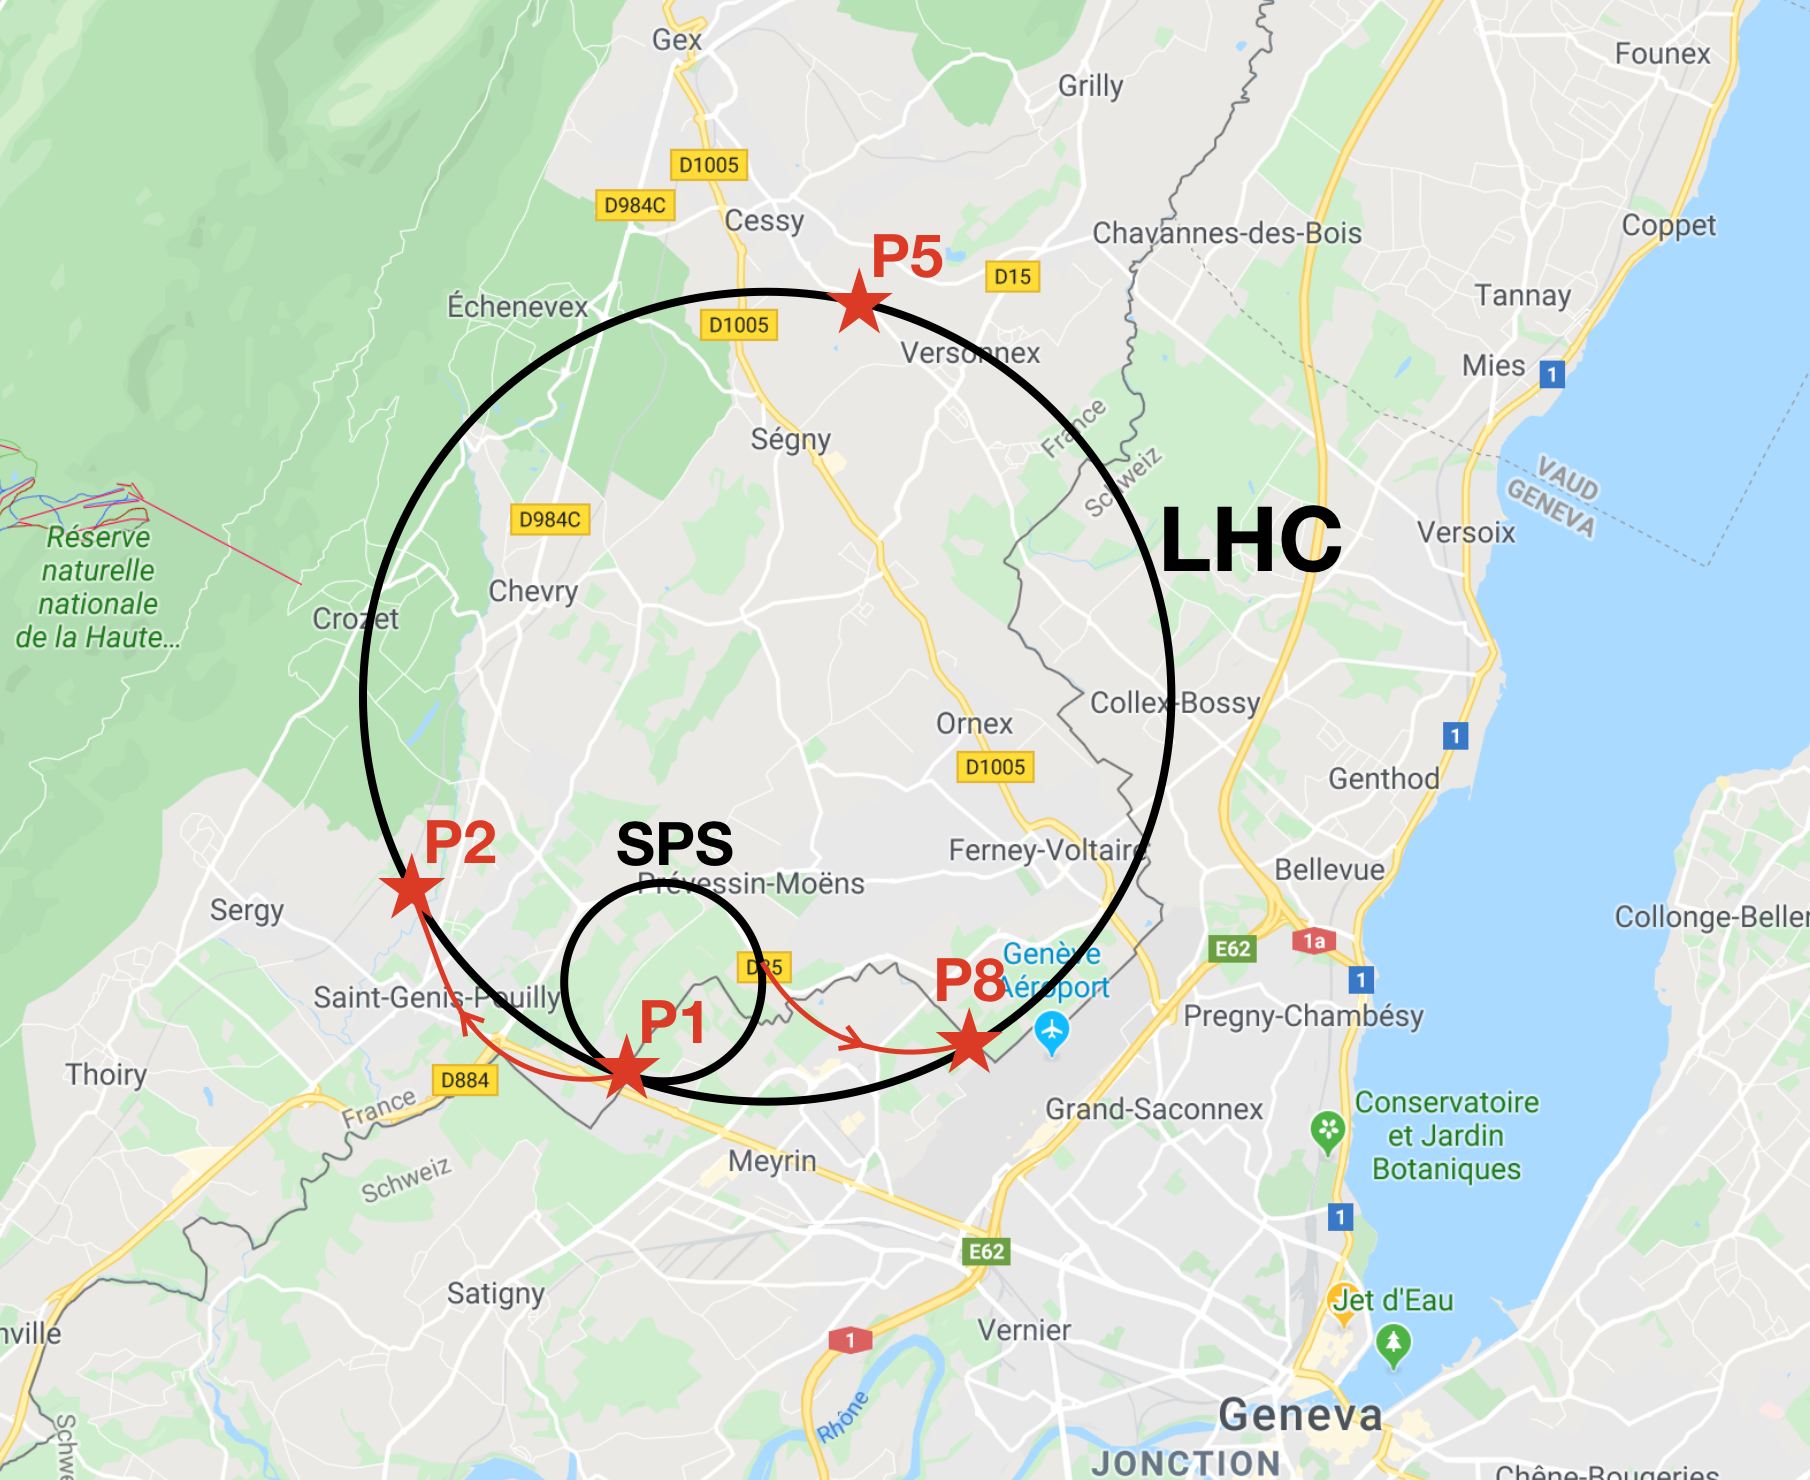
\includegraphics[width=0.48\textwidth,keepaspectratio]{figures/lhc/lhc_drawn_on_map_withpoints.png}
    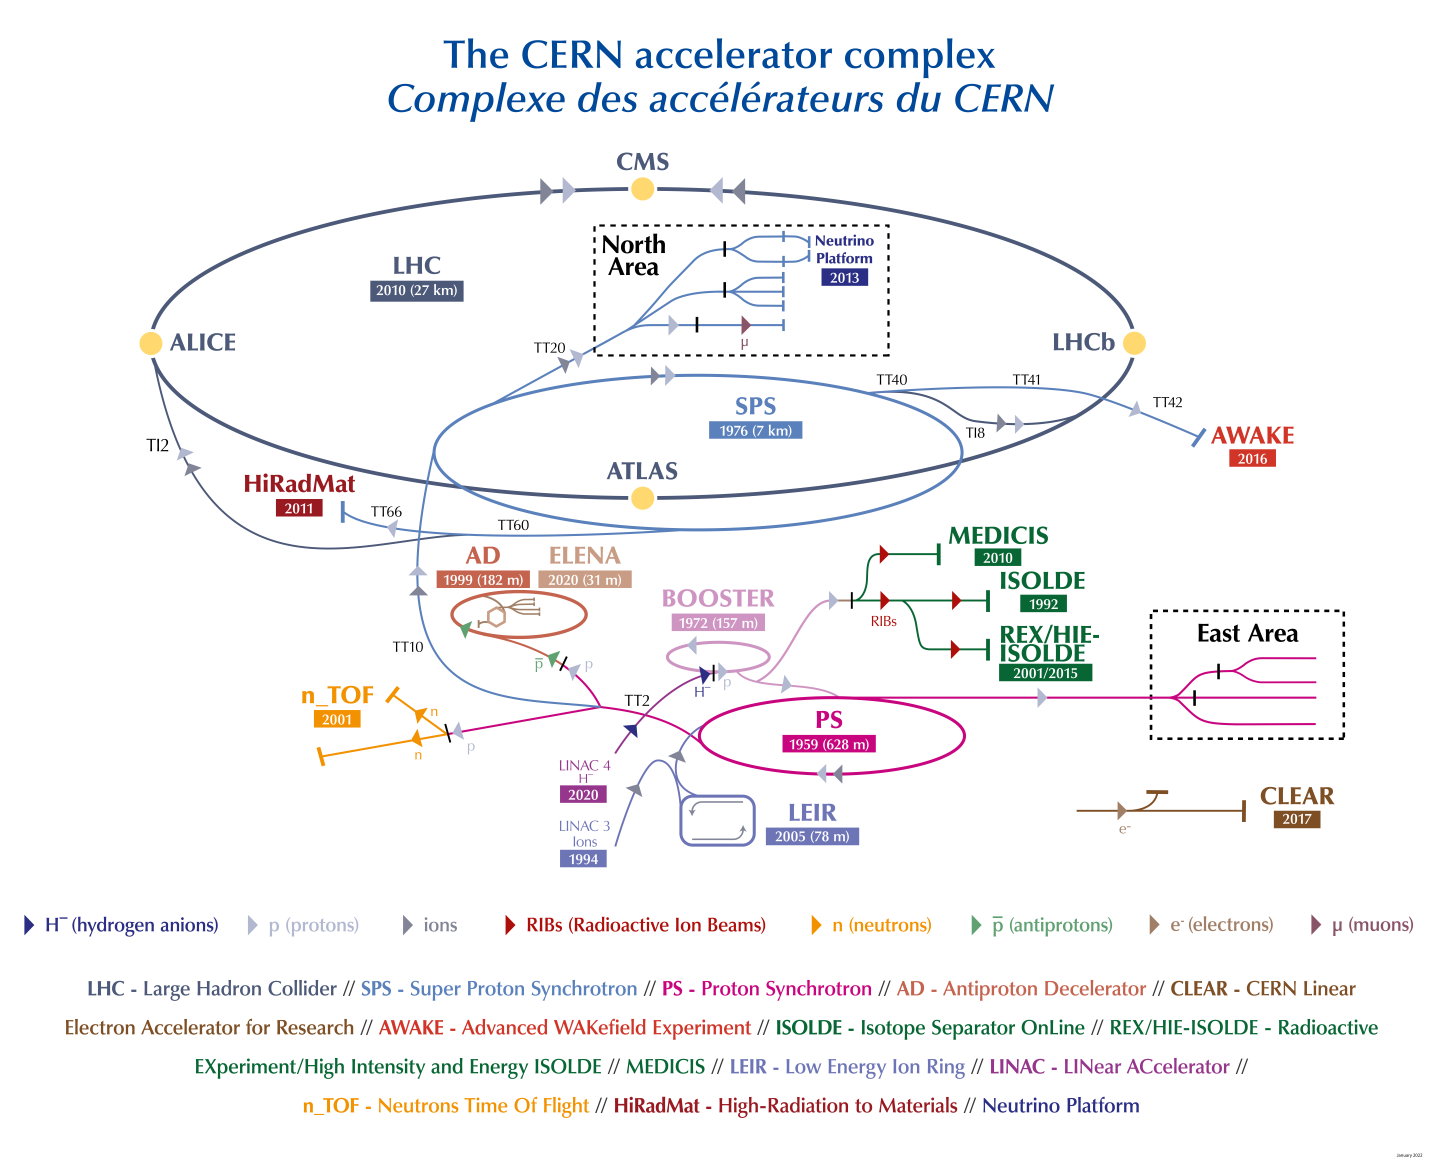
\includegraphics[width=0.48\textwidth,keepaspectratio]{figures/lhc/cern_complex.png}
        \caption{
        (Left) The LHC ring (bigger ring) and the Super Proton Synchrotron (smaller ring) with the nearby town of Geneva for size comparison. 
        The four red stars indicate the \pp collision points. 
        (Right) The accelerator complex at CERN.
        } 
        \label{fig:lhc_on_map_and_complex}
    \end{figure}
%%%%%%%%%%%%%%%%%%%%
For reference, the inscribed area of the LHC (56.7$\Km^{2}$) is almost four times greater than the area of the neighboring city of Geneva (15.9$\Km^{2}$).

The LHC is not only a particle \emph{accelerator} but also a proton-proton (\pp), proton-lead ion, and lead-lead ion \emph{collider}.
By sending one particle beam clockwise around the ring and the other beam counterclockwise, the charged particles are carefully maneuvered around the ring using dipole magnets and collimated into tight proton \emph{bunches} using quadrupole magnets before they ultimately collide at 4 specific points along the LHC, as shown in Fig.~\ref{fig:lhc_on_map_and_complex} (Left, red stars).
% , anywhere from , , and sandwiched between the scenic Jura mountains to the west and the sprawling city of Geneva (Genève) to the east
%  straddles the Franco-Swiss border, approximately 100\meter below the surface of the earth (Fig.~\ref{fig:lhc_and_boosters}, Left).
When the LHC is fully powered, \emph{each} proton in the beam carries an average energy of 6.5\TeV which gives a single \pp collision a center-of-mass energy of 13\TeV.
This emulates the conditions theorized to exist at the beginning of the universe, which allows cosmological studies to be carried out.
The hugely energetic \pp collisions cause the quark and gluon constituents within the protons to interact with each other and transform into new particles.
The newly created particles and the residual particle debris are ejected away from the collision point---whether straight down the beampipe, completely orthogonal to it, or somewhere in between.
A massive particle detector is stationed at each of the 4 collision points to detect the outgoing particle ``spray''.
The 4 main particle detectors and their locations along the LHC are:
\begin{itemize}
    \item A Toroidal LHC ApparatuS (ATLAS)---located at the first collision point (P1),
    \item A Large Ion Collider Experiment (ALICE)---located at P2,
    \item the Compact Muon Solenoid (CMS, Chapter~\ref{ch:cms}) experiment---located at P5, and
    \item the LHC-beauty (LHCb) experiment---located at P8.
\end{itemize}
% ATLAS	A Toroidal LHC Apparatus
% CMS	Compact Muon Solenoid
% LHCb	LHC-beauty
% ALICE	A Large Ion Collider Experiment
% TOTEM	Total Cross Section, Elastic Scattering and Diffraction Dissociation
% LHCf	LHC-forward
% MoEDAL	Monopole and Exotics Detector At the LHC
% FASER	ForwArd Search ExpeRiment
% SND	Scattering and Neutrino Detector

The world-renowned feat of the digging, constructing, commissioning, and monitoring of the LHC was made possible by CERN:
% - Before the LHC, LEP was originally in the tunnel.
%     - LEP ran from TODO--TODO.
the European Organization for Nuclear Research (French: \emph{Conseil Européean pour la Recherche Nucléaire}).
CERN is an international collaboration of---at the time of this writing---more than 33 countries,
% it's actually 34.
% Learn about the series of accelerators here:
% https://cdsweb.cern.ch/record/2771424/files/CERNAnnualReport_2020_EN.pdf
each of which is considered either a Member State, an Associate Member State, or an Observer.
The complex of CERN (Fig.~\ref{fig:lhc_on_map_and_complex}, Right) is located just to the west of P1 and is akin to a small science \emph{city}---complete with many offices, manufacturing facilities, and experiments such as the Antiproton Decelerator (AD), the Neutrons Time of Flight (n$\_$TOF), and the Isotope Separator OnLine (ISOLDE) experiments.
% the world's largest and most powerful particle accelerator, the Large Hadron Collider (LHC).
% The completion of this world-renowned feat was only possible through the careful efforts of thousands of scientists, engineers, administrators, \etc from all over the world.
% At the time of this writing, CERN is associated with at least 33 countries, each of which is considered either a Member State, an Associate Member State, or an Observer.
Although the LHC is the most famous of the accelerators at CERN, its fame is only made possible by a series of smaller and lesser-known accelerators that \emph{feed} the LHC.
% would not be able to accelerate \emph{any} charged particles from rest; not collide particles at such massive energies if not for the lesser-known accelerators that feed into the LHC.
% but it takes clever engineering and a series of smaller accelerators to eventually feed particles into the LHC to reach their maximum energy of 6.5\TeV.
Therefore, a natural way to explore the intricacies and inner workings of the LHC is to follow the path of one of its ``inhabitants''---a single proton---as it makes its way to and through the gigantic collider.

\section{The Journey of a Proton at the LHC}
The journey to discovery begins in a surprisingly small tank of hydrogen gas (\htwo) located in the LINAC4 building at the main CERN site.
% , in which a proton that is bound to another proton as a molecule of H2 .
% Pic of hydrogen source from here: https://www.lhc-closer.es/taking_a_closer_look_at_lhc/0.linac4
Inside this tank, a proton---conveniently called \pname---and approximately 1\tentothe{11} other protons coexist in bound states as molecules of H2.
Although the tank has a meager mass of TODO\Kg, it has enough protons inside to keep the LHC RUNNING for over 200\,000 years of constant operation.

Protons get injected into Series of smaller accelerators
    - The \emph{Linac4}---a linear particle accelerator---accelerates hydride ions (H$^-$) to 160\MeV which eventually make their way into the \emph{Proton Synchrotron Booster} (PSB).
    - In the PSB, each hydride ion has its electron pair completely stripped away, leaving only the bare proton TODO: mention electric field?
    - The protons then enter a series of circular accelerators, each machine feeding protons into the next while increasing the proton com energy by at least 1 order of magnitude.
    - The flow 
    - These protons are then accelerated to 2\GeV at which point they are injected into the \emph{Proton Synchrotron} (PS).
    - The PS then increases the proton energy to 26\GeV to be fed into the \emph{Super Proton Synchrotron} (SPS).
    - The penultimate step is for the SPS to further energize the protons to 450\GeV a accelerates protons to com energy
Finally the protons enter the LHC.

Protons are further accelerated to the maximum energy of 6.5\TeV using RF cavities to kick them.
- The protons would 
- 1232 dipole magnets made of copper-clad niobium-titanium are used to turn the proton beams.
- 392 TODO: 506? quadrupole magnets compress the proton bunches to make them more linear.
- The cryogenics of the 96\tonne of superfluid helium-4

Finally the proton bunches approach a collision point.
- Beam pipes are conjoined in an ``X'' shape (Fig. TODO) where 2 proton bunches cross---a \emph{bunch crossing} (BX).
- Out of more than 40 million \pp collisions that could have occurred, a mere 50 collisions take place on average (\ie only 0.000\,1\%).
    - This is a testament to just how small protons truly are.
- Frequency of BX: considering that proton bunches are spaced 25\ns apart, this means 
Just as the PS feeds protons into the SPS, which feeds protons into the LHC, so too is it being considered for the LHC to feed a new project---the 100\Km Future Circular Collider.

In the event that \pname does not collide with any of the oncoming protons, then it is simply ``recycled'' and continues going around the LHC ring for another opportunity at a \pp collision.


SPECS
- Luminosity
- rates
- data

N obs events = xs * eff * Lint 
cross section is specific to the process
efficiency is ideally unity.

\section{High-Luminosity LHC}




Contrary to what some people may think, protons are not sent one by one at each other, hoping for a collision.
% they are simply too small to precisely aim at one another and hope for a collision.
Instead 100 billion protons are packed together into a ``proton bunch''.
A single proton bunch is about the size of a human hair ($\approx$50\mum wide and $\approx$10\cm long). 
The clockwise and counterclockwise rings are filled to a maximum of 2808 proton bunches, each one spaced 25\ns apart, and then sent to collide. 

It requires an incredibly strong magnetic field to turn the protons as they make their revolutions around the LHC. 
Recall that charged particles bend in a magnetic field, via the Lorentz force. 
Therefore, the LHC is equipped with 1232 dipole magnets distributed all along the length of the beam pipe to keep the proton bunches turning in the tunnel.
The cross section of such a dipole magnet is shown in Fig.~\ref{fig:lhc_dipole_xs}.
Each dipole magnet is 14.3\meter long, weighs 35\tonne, cost nearly 500\,KCHF to produce, and has nearly 11\,700 amps of current running through it. 
Only with such massive currents is it possible to generate the appropriate magnetic field strength of 8\tesla to keep the protons turning. 
The magnetic field is maintained by titanium-niobium coils, which are kept under cryogenic conditions using liquid helium to achieve the necessary temperature of 1.9\kelvin to reach a superconducting state; 
this temperature is colder than that of outer space!
%%%%%%%%%%%%%%%%%%%%
\begin{figure}[pbth]
\centering
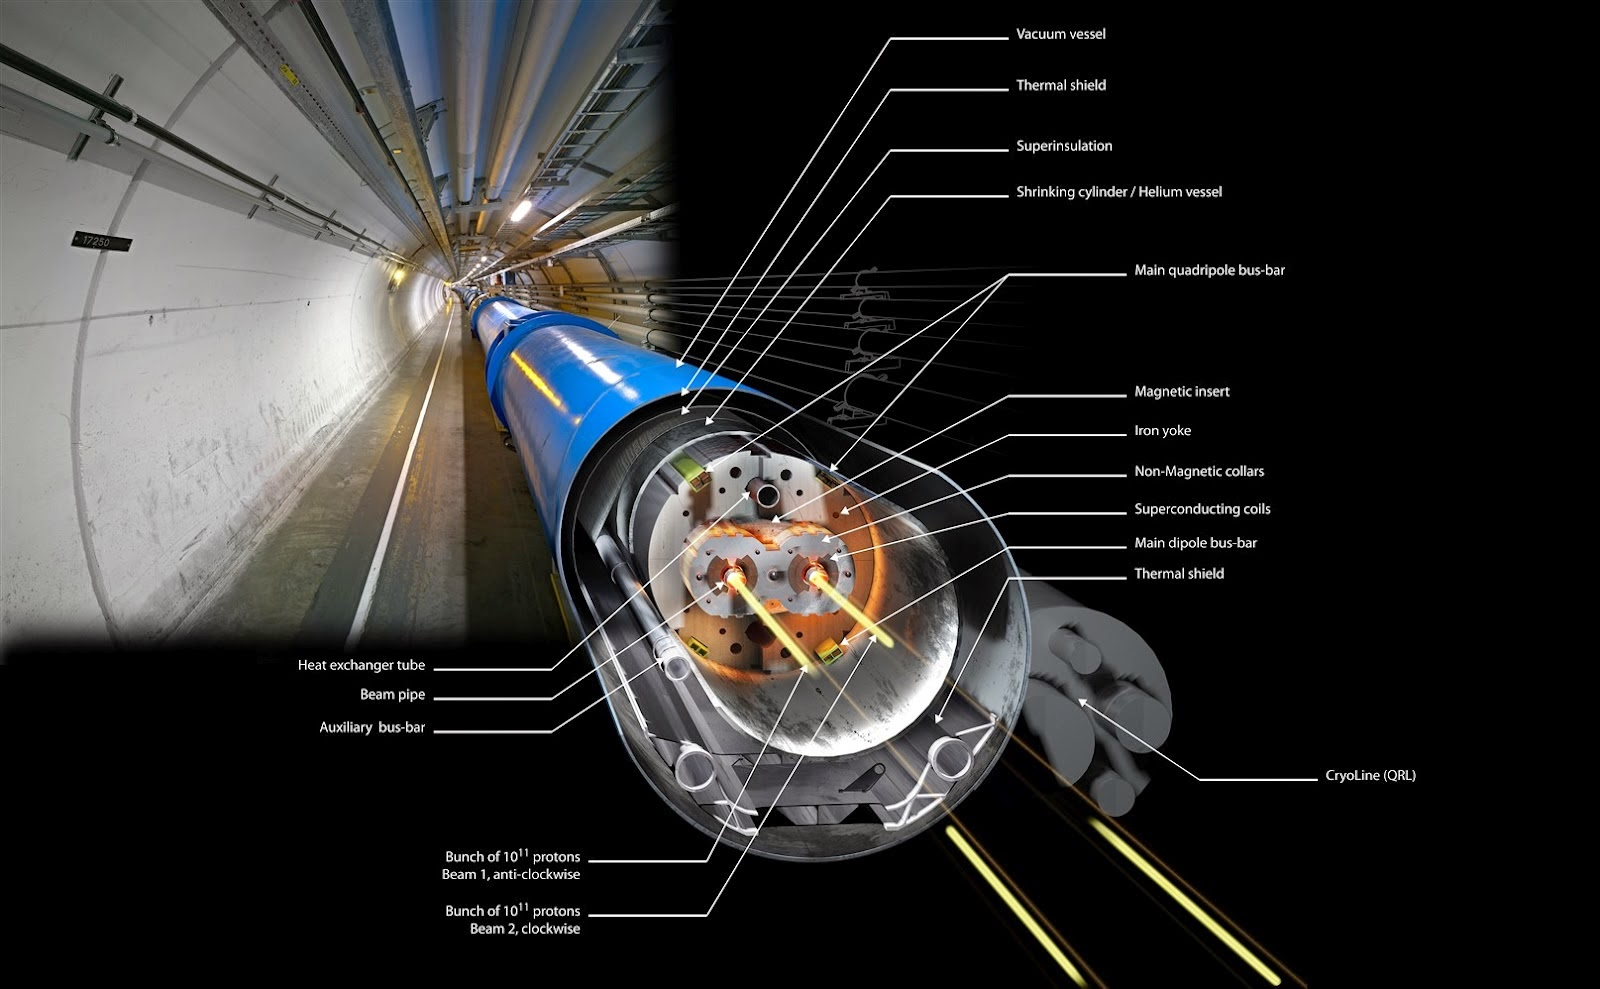
\includegraphics[width=15cm,height=10cm,keepaspectratio]{figures/lhc/lhc_dipole_xs.jpg}
    \caption{
    A cross section of one of the 1232 dipole magnets which span the entire length of the LHC tunnel.} 
    \label{fig:lhc_dipole_xs}
\end{figure}
%%%%%%%%%%%%%%%%%%%%

% proton is a {\it hadron} collider 
% It is fed by the Super Proton Synchrotron 
There are only four specific ``Points'' along the LHC where the proton bunches actually cross, as shown in Fig.~\ref{fig:lhc_on_map_and_complex} (Left, red stars).
At each of these four points, there is a unique and gigantic particle detector to catch all the decay products from the \pp collisions. 

% LPS SPS
% into a beam pipe going clockwise and another 2800 bunches going around counterclockwise, 
As the two bunches are just about to cross one another, they are squeezed down using quadrupole magnets, focusing the beams more tightly, increasing their chance for tasty \pp collisions.
%from 50 $\mu$m
During such a bunch crossing (BX), amazingly most of the protons just pass right by one another; 
out of the possible 100 billion possible collisions that could have occurred, Fig.~\ref{plt:pileup} shows that on average only 32 collisions occurred per BX in the LHC 2018 run, according to a particle detector called CMS, described in Chapter~\ref{ch:cms}.
It should be mentioned that the luminosity of the LHC is on the order of \LHigh. %$10^{34}$ Hz/cm$^2$.
%%%%%%%%%%%%%%%%%%%%
\begin{figure}[pbth]
\centering
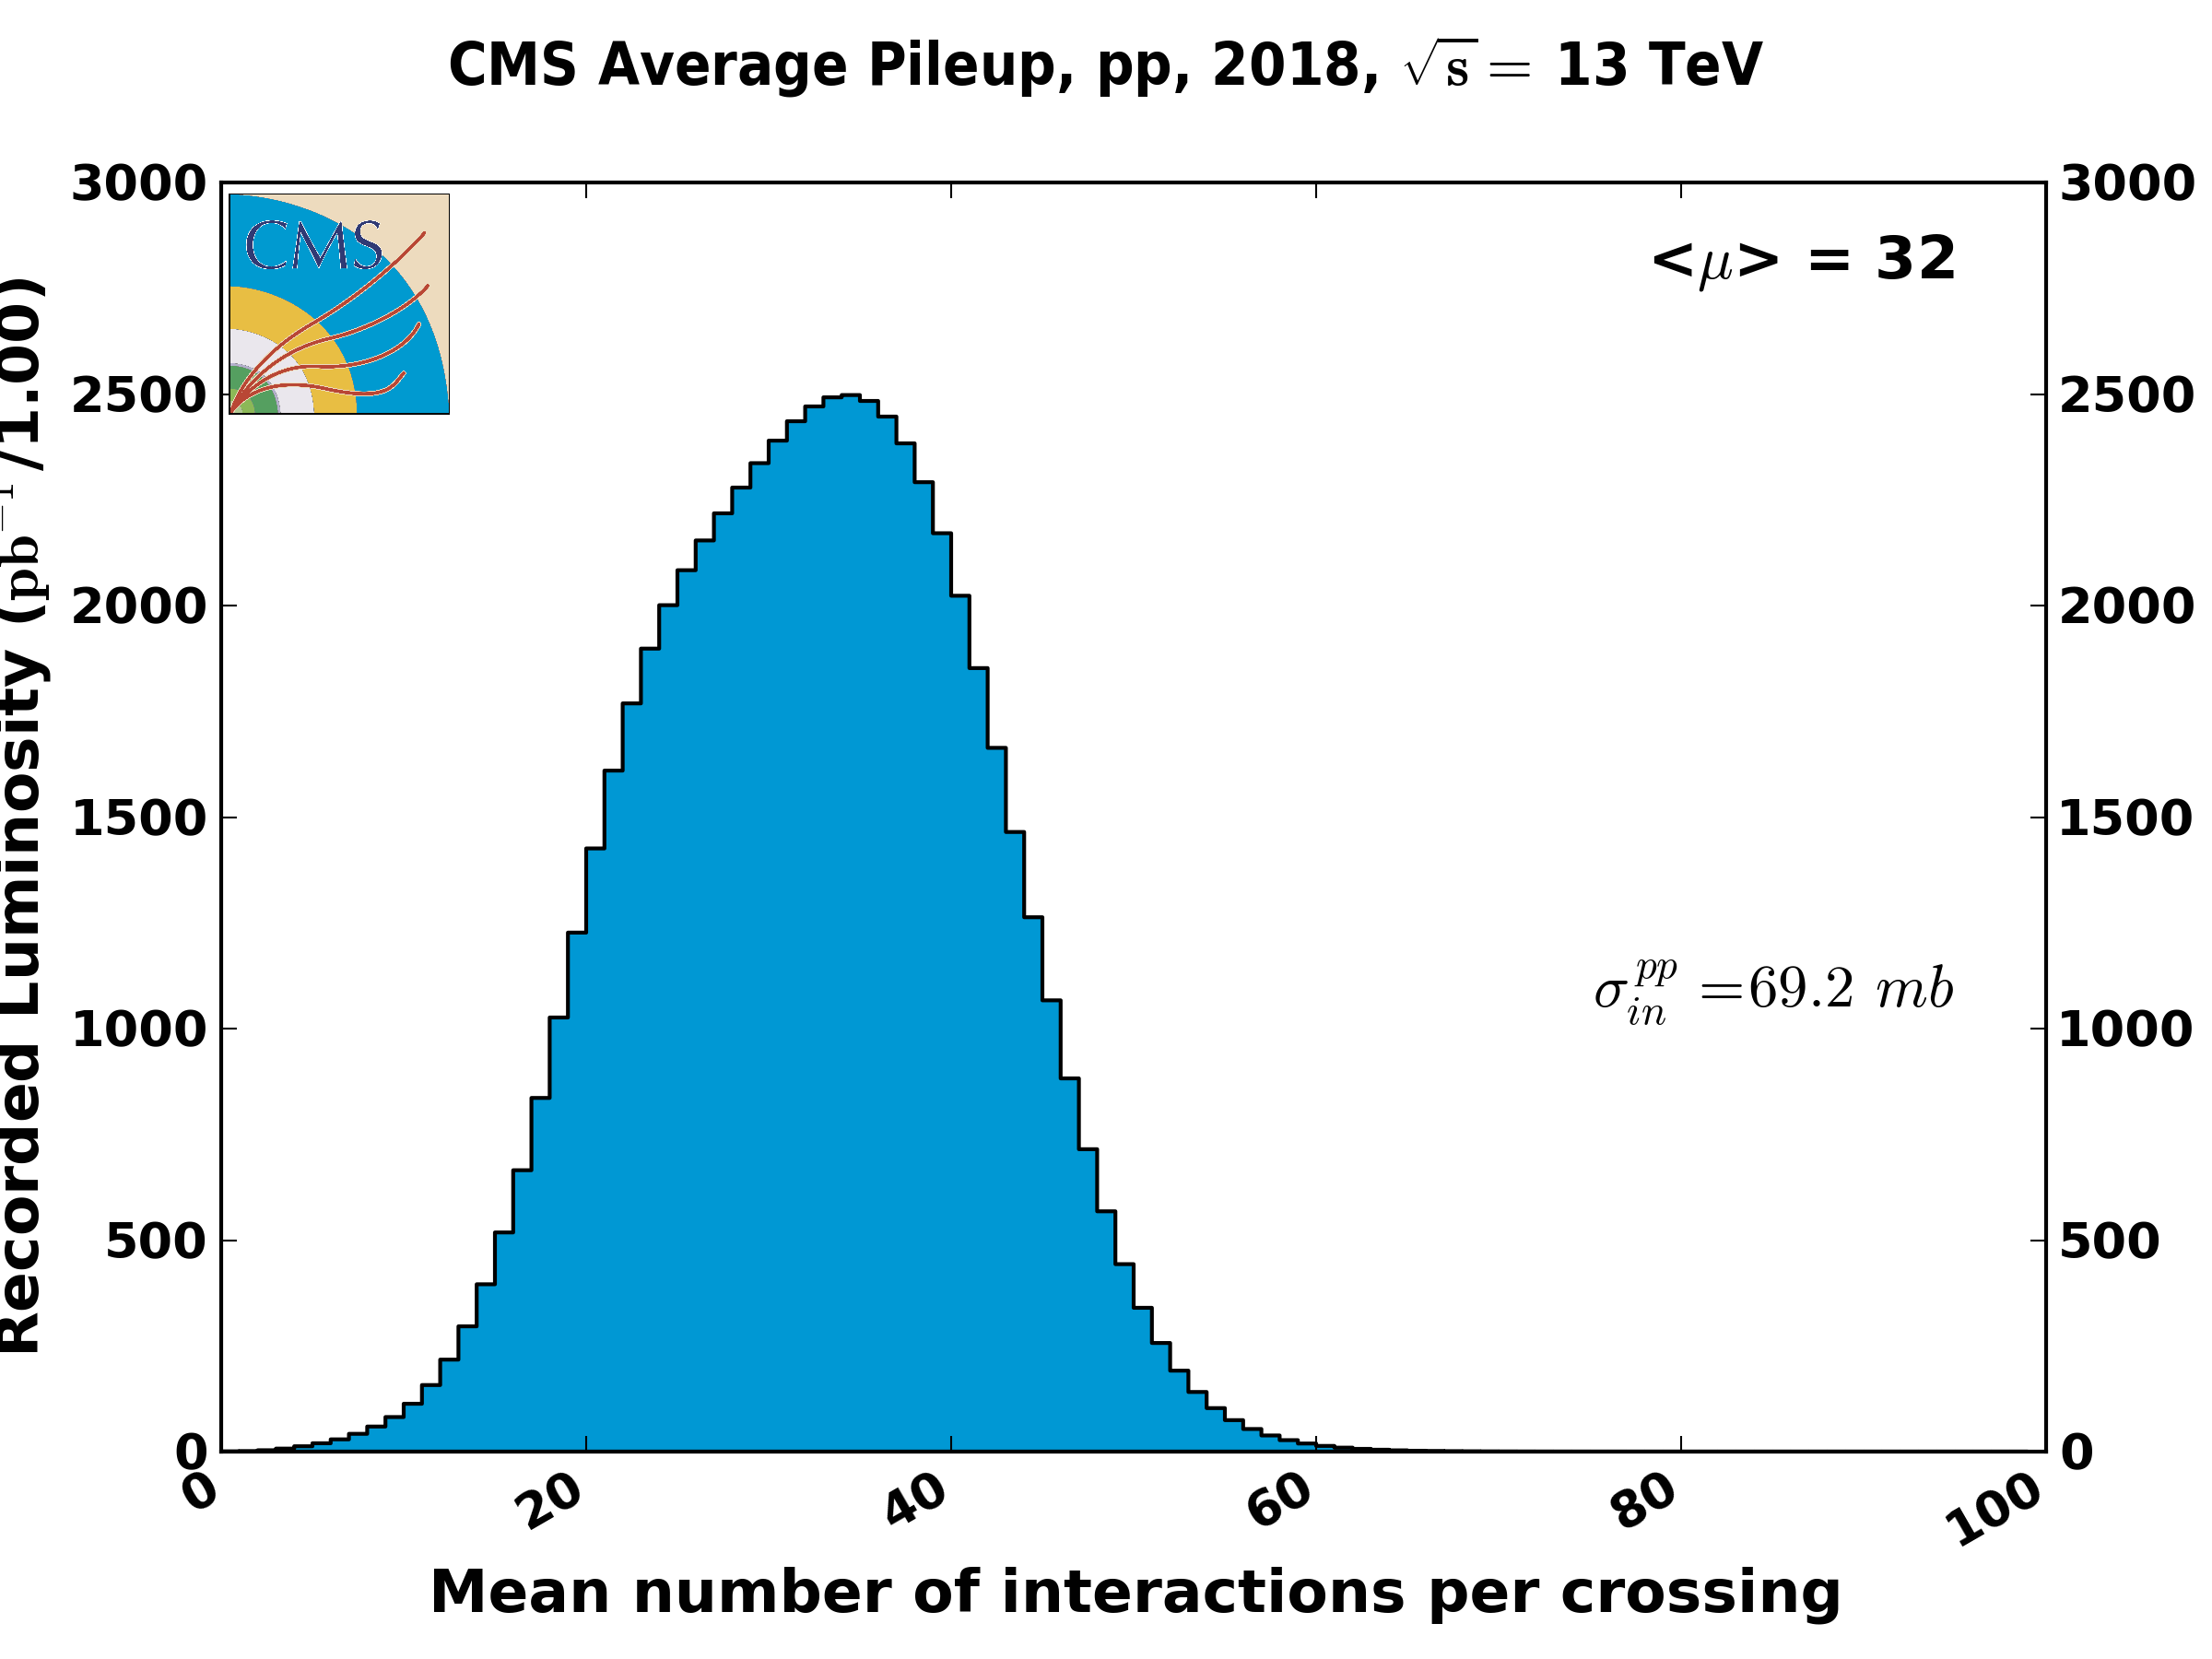
\includegraphics[width=10cm,height=10cm,keepaspectratio]{figures/lhc/pileup_pp_2018.png}
    \caption{Histogram showing the distribution of the average number of \pp collisions per proton bunch crossing (pile up) which CMS recorded during the LHC 2018 run.} 
    \label{plt:pileup}
\end{figure}
%%%%%%%%%%%%%%%%%%%%

As the proton bunches whiz around the LHC, they are given ``kicks'' from radio-frequency (RF) cavities, which accelerate the protons to a max speed of 99.999996\%$c$.
It is analgous to the timing required when pushing someone on a swing: push at just the right time to increase their momentum.
At this speed, \emph{each proton} carries 6.5\TeV of energy, such that a single \pp collision contains a monstrous center-of-mass energy of $\sqrt{s} = 13\TeV$:
more than enough energy to create new particles like top quarks, Higgs bosons, and potentially BSM particles.
%%%%%%%%%%%%%%%%%%%%
\begin{figure}[pbth]
    \centering
    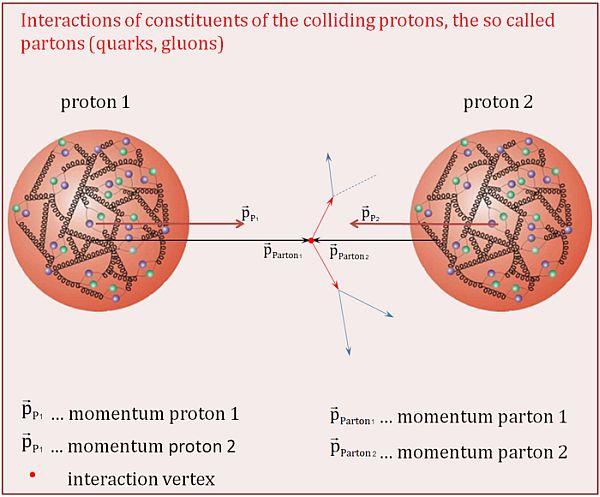
\includegraphics[width=10cm,height=10cm,keepaspectratio]{figures/lhc/proton_proton_quarksandgluons.jpg}
        \caption{
        Two protons can be smashed together at very high energies to have their partons interact and convert the high energies into new kinds of matter.} 
        \label{fig:pp_collision}
    \end{figure}
    %%%%%%%%%%%%%%%%%%%%
% The LHC has ushered in the era of ``TeV-scale physics'',
% exploring the 
% - which is about the same amount of energy of a really fat flying mosquito.
In order to ``see'' such interesting particles, one needs to detect the outgoing particles produced from \pp collisions;
one needs a dedicated \emph{particle detector}...
The Compact Muon Solenoid detector should do the trick.
% It takes a proton \~90 $\mu$s 
% to make a complete revolution around the LHC moving at such a speed.

% \chapter{The Large Hadron Collider}  % Automatically turned into all caps.
% \label{ch:lhc}

% Located on the border between France and Switzerland, sandwiched between the beautiful Jura mountains to the west and the sprawling city of Geneva (Genève) to the east, is CERN:
% the European Organization for Nuclear Research 
% (Conseil Européean pour la Recherche Nucléaire).
% CERN is an international collaboration of more than 23 member states and its ``family'' is steadily growing.
% This collaboration is responsible for the construction and commissioning of the world's largest and most powerful particle accelerator:
% the Large Hadron Collider (LHC).

% The LHC collides particles using the brightest beams and highest energies that humans have ever made.
% Bright beams meaning highest luminosity.

% Higgs boson produced every 1 billion collisions.

% Beginning in 2026 (FIXME), the LHC will undergo a ``Phase 2'' upgrade and become the High-Luminosity LHC.
% This upgrade will increase the collider's luminosity by 10 fold (FIXME) and is predicted to deliver SO much data 3000 fb?.
